\newcommand{\tikzBGSS}{
\begin{tikzpicture}[very thick, node distance=2.2cm, >=latex]
  % Latent states
  \node[latent, fill, minimum size=38pt] (z0) {$z_{t}$};
  \node[latent, right=of z0, minimum size=38pt, xshift=2.2cm] (z1) {$z_{t+1}$};

  % Observations
  \node[obs, below=1.4cm of z0, fill, minimum size=38pt] (o0) {$v_{t}$};
  \node[obs, below=1.4cm of z1, fill, minimum size=38pt] (o1) {$v_{t+1}$};

  % Continuation anchors
  \coordinate[left=1.2cm of z0] (cstart);
  \coordinate[right=1.2cm of z1] (cend);

  % Edges: latent dynamics (forward/generative)
  \edge {z0} {z1}

  % Edges: emissions (forward/generative)
  \edge {z0} {o0}
  \edge {z1} {o1}

  % Inference direction (backward/curved dotted arrows)
  \draw[dashed, ->, >=stealth, color=blue!60, thick, bend left=35] (o0) to (z0);
  \draw[dashed, ->, >=stealth, color=blue!60, thick, bend left=35] (o1) to (z1);

  % Dashed time continuation
  \draw[dashed] (cstart) -- (z0);
  \draw[dashed] (z1) -- (cend);

  % --- Annotations (show only one edge per type for clarity) ---
  % State transition conditional distribution (only first edge)
  \draw[draw=none] (z0) -- node[midway, above=0pt, font=\normalsize] {$z_{t+1} \mid z_t \sim \mathcal{N}({\color{black}\bar{a}_t} z_t, {\color{blue}\bar{p}_t})$} (z1);

  % Observation conditional distribution (only first edge)
  \draw[draw=none] (z0) -- node[midway, right=2pt, font=\normalsize] {$v_t \mid z_t \sim \mathcal{N}({\color{black}k_t} z_t, {\color{blue}(\Lambda_t^{v})^{-1}})$} (o0);

  % Inference label (on curved arrow)
  \draw[draw=none] (o0) -- node[midway, left=8pt, font=\normalsize, color=blue!70] {\textbf{inference}} (z0);

  % Legend box for poster (commented out for now)
  % \node[draw=black, thick, fill=white, rectangle,
  %       inner sep=6pt, font=\small, anchor=north east]
  %       at ($(z2.north east)+(0.5,0.8)$) {
  %   \begin{tabular}{l}
  %     {\color{teal!70!black}\rule{0.8ex}{0.8ex}} Model Parameters \\
  %     {\color{red!80}\rule{0.8ex}{0.8ex}} Uncertainty Parameters
  %   \end{tabular}
  % };
\end{tikzpicture}
}

\newcommand{\tikzMambaSSM}{
\begin{tikzpicture}[very thick, node distance=2.2cm, >=latex]
  % Input tokens (control signals) - TOP ROW
  \node[obs, fill, minimum size=38pt] (u0) {$u_{t-1}$};
  \node[obs, right=of u0, minimum size=38pt, xshift=2.2cm] (u1) {$u_{t}$};

  % Latent states - BOTTOM ROW
  \node[latent, below=1.4cm of u0, fill, minimum size=38pt] (z0) {$z_{t-1}$};
  \node[latent, below=1.4cm of u1, fill, minimum size=38pt] (z1) {$z_{t}$};

  % Continuation anchors
  \coordinate[left=1.2cm of u0] (cstart_u);
  \coordinate[right=1.2cm of u1] (cend_u);
  \coordinate[left=1.2cm of z0] (cstart_z);
  \coordinate[right=1.2cm of z1] (cend_z);

  % Edges: state transitions (horizontal)
  \edge {z0} {z1}

  % Edges: control inputs drive states (VERTICAL downward)
  \edge {u0} {z0}
  \edge {u1} {z1}

  % Dashed time continuation (only for states)
  \draw[dashed] (cstart_z) -- (z0);
  \draw[dashed] (z1) -- (cend_z);

  % --- Annotations (show only one edge for clarity) ---
  % State transition equation (only first edge)
  \draw[draw=none] (z0) -- node[midway, below=0pt, font=\normalsize] {$z_t = {\color{black}\bar{A}_t} z_{t-1} + {\color{black}\bar{B}_t} u_t$} (z1);

  % Control signal label (vertical arrow)
  \draw[draw=none] (u1) -- node[midway, right=2pt, font=\normalsize] {\textbf{control inputs}} (z1);
\end{tikzpicture}
}

% KLA Pipeline: Stochastic → Bayesian → Parallel (3-column overview figure)
\newcommand{\tikzKLAPipeline}{
\begin{tikzpicture}[
    header/.style={font=\small\bfseries},
    eqn/.style={font=\small},
    arrow/.style={->, thick, >=stealth},
    wiggly/.style={decorate, decoration={snake, amplitude=0.4mm, segment length=2.5mm}, ->, thick, >=stealth},
    node distance=0.6cm
]

% === Column 1: Continuous-Time (Graphical Model) ===
\begin{scope}[local bounding box=col1]
  % Latent states
  \node[latent, minimum size=20pt] (z0) {$z_{t-1}$};
  \node[latent, right=1.0cm of z0, minimum size=20pt] (z1) {$z_t$};

  % Observations
  \node[obs, below=0.8cm of z0, minimum size=20pt] (v0) {$v_{t-1}$};
  \node[obs, below=0.8cm of z1, minimum size=20pt] (v1) {$v_t$};

  % Edges - wiggly for stochastic transition (SDE noise)
  \draw[wiggly] (z0) -- (z1);
  \edge {z0} {v0}
  \edge {z1} {v1}

  % SDE annotation
  \node[below=0.5cm of v0, anchor=north, eqn, xshift=0.5cm] (sde) {
    $\mathrm{d}z = -az\,\mathrm{d}t + {\color{red!80}p}\,\mathrm{d}W$
  };
\end{scope}

% Column 1 header
\node[header, above=0.5cm of col1] (h1) {Continuous-Time};
\node[font=\scriptsize, below=-0.1cm of h1] {(OU Process)};

% === Column 2: Discrete-Time (Equations) ===
\begin{scope}[xshift=5.0cm, local bounding box=col2]
  \node[eqn, align=left] (trans) {
    $z_t \mid z_{t-1} \sim \mathcal{N}(\bar{a} z_{t-1},\, {\color{red!80}\bar{p}})$
  };
  \node[eqn, below=0.25cm of trans, align=left] (obs) {
    $v_t \mid z_t \sim \mathcal{N}(k z_t,\, {\color{red!80}(\Lambda^{\mathrm{v}})^{-1}})$
  };
  \node[eqn, below=0.5cm of obs, align=left, font=\scriptsize] (disc) {
    $\bar{a} = e^{-a\Delta t}$, \quad
    ${\color{red!80}\bar{p}} = \tfrac{p^2}{2a}(1-e^{-2a\Delta t})$
  };
\end{scope}

% Column 2 header
\node[header, above=0.5cm of col2] (h2) {Discrete-Time};
\node[font=\scriptsize, below=-0.1cm of h2] {(Gaussian SSM)};

% === Column 3: Inference (Scan) ===
\begin{scope}[xshift=10.5cm, local bounding box=col3]
  % Möbius matrices
  \node[draw, thick, minimum width=0.6cm, minimum height=0.6cm, font=\scriptsize] (m1) {$M_1$};
  \node[right=0.1cm of m1, font=\small] (circ1) {$\circ$};
  \node[draw, thick, minimum width=0.6cm, minimum height=0.6cm, right=0.1cm of circ1, font=\scriptsize] (m2) {$M_2$};
  \node[right=0.1cm of m2, font=\small] (dots) {$\cdots$};
  \node[draw, thick, minimum width=0.6cm, minimum height=0.6cm, right=0.1cm of dots, font=\scriptsize] (mt) {$M_T$};

  % Scan box
  \node[draw, thick, fill=green!10, rounded corners, below=0.5cm of m2, minimum width=2.2cm, font=\scriptsize] (scan) {
    \texttt{assoc\_scan}
  };

  % Output
  \node[eqn, below=0.35cm of scan, font=\scriptsize] (output) {
    ${\color{red!80}\lambda_t} = \frac{\alpha\lambda_{t-1}+\beta}{\gamma\lambda_{t-1}+\delta}$
  };

  % Arrow to scan
  \draw[arrow] (m2.south) -- (scan.north);
\end{scope}

% Column 3 header
\node[header, above=0.5cm of col3] (h3) {Inference};
\node[font=\scriptsize, below=-0.1cm of h3] {(M\"obius Scan)};

% === Arrows between columns ===
\draw[arrow, thick] ([xshift=0.4cm]col1.east) -- node[above, font=\scriptsize] {discretize} ([xshift=-0.4cm]col2.west);
\draw[arrow, thick] ([xshift=0.4cm]col2.east) -- node[above, font=\scriptsize] {Kalman} ([xshift=-0.4cm]col3.west);

% === Legend ===
\node[below=0.8cm of col2, font=\scriptsize] (legend) {
  \textbf{Legend:} black = shared with Mamba \quad {\color{red!80}\textbf{red}} = KLA-only (uncertainty)
};

\end{tikzpicture}
}

% GAUSS Language Model Architecture (for poster) - Bottom-to-Top layout
\newcommand{\tikzGAUSSArchitecture}{
\begin{tikzpicture}[
    box/.style={draw, thick, rounded corners=4pt, minimum width=3.8cm, minimum height=0.9cm, align=center, font=\normalsize},
    arrow/.style={->, thick, >=stealth},
    node distance=0.8cm
]
  % Input tokens (BOTTOM)
  \node[box, fill=gray!15] (input) {Input Tokens};

  % Embedding
  \node[box, fill=blue!8, above=of input] (embed) {Embedding};

  % MLP
  \node[box, fill=blue!8, above=of embed] (mlp) {MLP};

  % GAUSS Block with ×N
  \node[box, fill=green!15, above=of mlp, minimum height=1.1cm] (gauss) {GAUSS Block\\[-2pt]{\small (Kalman Filter)}};
  \node[right=0.4cm of gauss, font=\large] {$\times N$};

  % Midpoint for μ, Σ label
  \coordinate[above=1.0cm of gauss] (midpoint);

  % Logits Decoder (TOP)
  \node[box, fill=orange!15, above=2.2cm of gauss] (decoder) {Logits Decoder};

  % Arrows: standard flow (upward)
  \draw[arrow] (input) -- (embed);
  \draw[arrow] (embed) -- (mlp);
  \draw[arrow] (mlp) -- (gauss);

  % Arrow with μ, Σ label after GAUSS block
  \draw[->, thick, >=stealth] (gauss.north) -- node[right=3pt, font=\normalsize] {$\boldsymbol{\mu}, {\color{red!80}\boldsymbol{\Sigma}}$} (midpoint);

  % Wiggly arrow from midpoint to decoder with side label
  \draw[decorate, decoration={snake, amplitude=1.5mm, segment length=4mm}, ->, thick]
      (midpoint) -- (decoder.south)
      node[midway, right=0.6cm, align=left, font=\small] {Sample from $\mathcal{N}(\mu, \Sigma)$\\[2pt]\textbf{or}\\[2pt]Decode Mean $(\mu)$};

\end{tikzpicture}
}

% Hybrid OU Visualization: Timeline sample path + Graphical Model
% Two stacked panels connecting intuition (sample path) to inference structure (graphical model)
\newcommand{\tikzOUHybrid}{
\begin{tikzpicture}[
    every node/.style={font=\small},
    obs/.style={circle, draw, thick, fill=gray!40, minimum size=22pt, inner sep=1pt},
    latent/.style={circle, draw, thick, fill=white, minimum size=22pt, inner sep=1pt}
]

% === Panel 1: Timeline with OU sample path ===
\begin{scope}[local bounding box=timeline]
  % Axes
  \draw[->, thick] (0,0) -- (7.5,0) node[right] {$t$};
  \draw[->, thick] (0,-0.3) -- (0,2.2) node[above] {$x(t)$};

  % Uncertainty band (shaded region around mean)
  \fill[blue!8, opacity=0.6] plot[smooth, tension=0.7]
    coordinates {(0.3,2.0) (1.2,1.5) (2.2,1.0) (3.2,1.6) (4.2,1.3) (5.2,1.1) (6.2,1.5) (7.0,1.2)}
    -- plot[smooth, tension=0.7]
    coordinates {(7.0,0.8) (6.2,1.1) (5.2,0.7) (4.2,0.9) (3.2,1.2) (2.2,0.6) (1.2,1.1) (0.3,1.6)}
    -- cycle;

  % OU sample path (smooth curve with mean-reversion)
  \draw[thick, blue!70!black] plot[smooth, tension=0.7]
    coordinates {(0.3,1.8) (1.2,1.3) (2.2,0.8) (3.2,1.4) (4.2,1.1) (5.2,0.9) (6.2,1.3) (7.0,1.0)};

  % Mean level (dashed)
  \draw[dashed, gray] (0,1) -- (7.5,1) node[right, font=\scriptsize] {$\mu$};

  % Discrete sample points (on the OU path)
  \fill[red!80] (1.2,1.3) circle (2.5pt);
  \fill[red!80] (3.2,1.4) circle (2.5pt);
  \fill[red!80] (5.2,0.9) circle (2.5pt);

  % Time labels
  \node[below=1pt, font=\scriptsize] at (1.2,0) {$t_{k-1}$};
  \node[below=1pt, font=\scriptsize] at (3.2,0) {$t_k$};
  \node[below=1pt, font=\scriptsize] at (5.2,0) {$t_{k+1}$};

  % Tick marks
  \draw[thick] (1.2,0.05) -- (1.2,-0.05);
  \draw[thick] (3.2,0.05) -- (3.2,-0.05);
  \draw[thick] (5.2,0.05) -- (5.2,-0.05);

  % Panel label
  \node[font=\scriptsize\itshape, anchor=north west] at (0.1,2.1) {Continuous path};
\end{scope}

% === Panel 2: Graphical Model (below timeline) ===
\begin{scope}[yshift=-2.5cm, local bounding box=gm]
  % Latent nodes
  \node[latent] (z0) at (1.2,0) {$z_{k-1}$};
  \node[latent] (z1) at (3.2,0) {$z_k$};
  \node[latent] (z2) at (5.2,0) {$z_{k+1}$};

  % Observation nodes (moved to -1.3 for longer arrows)
  \node[obs] (v0) at (1.2,-1.3) {$v_{k-1}$};
  \node[obs] (v1) at (3.2,-1.3) {$v_k$};
  \node[obs] (v2) at (5.2,-1.3) {$v_{k+1}$};

  % State transition edges
  \draw[->, thick] (z0) -- (z1);
  \draw[->, thick] (z1) -- (z2);

  % Observation edges
  \draw[->, thick] (z0) -- (v0);
  \draw[->, thick] (z1) -- (v1);
  \draw[->, thick] (z2) -- (v2);

  % Continuation (dots)
  \node[font=\normalsize] at (0.3,0) {$\cdots$};
  \node[font=\normalsize] at (6.1,0) {$\cdots$};

  % Transition distribution label
  \node[above=3pt, font=\scriptsize] at (2.2,0) {$\mathcal{N}(\bar{a}z, {\color{red!80}\bar{q}})$};

  % Panel label (moved to y=0.7 to avoid overlap)
  \node[font=\scriptsize\itshape, anchor=north west] at (0.1,0.7) {Discrete model};
\end{scope}

% === Vertical connection lines (sample points to graphical model nodes) ===
\draw[dotted, gray, thick] (1.2,-0.1) -- (1.2,-2.25);
\draw[dotted, gray, thick] (3.2,-0.1) -- (3.2,-2.25);
\draw[dotted, gray, thick] (5.2,-0.1) -- (5.2,-2.25);

% === Caption / Legend ===
\node[below=0.2cm of gm, font=\scriptsize, align=center] {
  OU discretization: $\bar{a} = e^{-\lambda\Delta t}$, \quad
  ${\color{red!80}\bar{q}} = \tfrac{\sigma^2}{2\lambda}(1-e^{-2\lambda\Delta t})$
};

\end{tikzpicture}
}

% === Variant A: Wide layout (for figure*) ===
% tikzOUHybridWide: Adds Möbius Scan panel to the RIGHT of the Bayesian Network
\newcommand{\tikzOUHybridWide}{
\begin{tikzpicture}[
    every node/.style={font=\small},
    obs/.style={circle, draw, thick, fill=gray!40, minimum size=22pt, inner sep=1pt},
    latent/.style={circle, draw, thick, fill=white, minimum size=22pt, inner sep=1pt}
]

% === Panel 1: Timeline with OU sample path ===
\begin{scope}[local bounding box=timeline]
  % Axes
  \draw[->, thick] (0,0) -- (7.5,0) node[right] {$t$};
  \draw[->, thick] (0,-0.3) -- (0,2.2) node[above] {$x(t)$};

  % Uncertainty band (shaded region around mean)
  \fill[blue!8, opacity=0.6] plot[smooth, tension=0.7]
    coordinates {(0.3,2.0) (1.2,1.5) (2.2,1.0) (3.2,1.6) (4.2,1.3) (5.2,1.1) (6.2,1.5) (7.0,1.2)}
    -- plot[smooth, tension=0.7]
    coordinates {(7.0,0.8) (6.2,1.1) (5.2,0.7) (4.2,0.9) (3.2,1.2) (2.2,0.6) (1.2,1.1) (0.3,1.6)}
    -- cycle;

  % OU sample path (smooth curve with mean-reversion)
  \draw[thick, blue!70!black] plot[smooth, tension=0.7]
    coordinates {(0.3,1.8) (1.2,1.3) (2.2,0.8) (3.2,1.4) (4.2,1.1) (5.2,0.9) (6.2,1.3) (7.0,1.0)};

  % Mean level (dashed)
  \draw[dashed, gray] (0,1) -- (7.5,1) node[right, font=\scriptsize] {$\mu$};

  % Discrete sample points (on the OU path)
  \fill[red!80] (1.2,1.3) circle (2.5pt);
  \fill[red!80] (3.2,1.4) circle (2.5pt);
  \fill[red!80] (5.2,0.9) circle (2.5pt);

  % Time labels
  \node[below=1pt, font=\scriptsize] at (1.2,0) {$t_{k-1}$};
  \node[below=1pt, font=\scriptsize] at (3.2,0) {$t_k$};
  \node[below=1pt, font=\scriptsize] at (5.2,0) {$t_{k+1}$};

  % Tick marks
  \draw[thick] (1.2,0.05) -- (1.2,-0.05);
  \draw[thick] (3.2,0.05) -- (3.2,-0.05);
  \draw[thick] (5.2,0.05) -- (5.2,-0.05);

  % Continuous-time SDE
  \node[font=\scriptsize, anchor=north west] at (3.5,2.4) {$\mathrm{d}x = -a(x-\mu)\mathrm{d}t + \sigma\mathrm{d}W$};

  % Panel label
  \node[font=\scriptsize\itshape, anchor=north west] at (0.1,2.4) {Continuous path};
\end{scope}

% === Panel 2: Graphical Model (below timeline) ===
\begin{scope}[yshift=-2.5cm, local bounding box=gm]
  % Latent nodes
  \node[latent] (z0) at (1.2,0) {$z_{k-1}$};
  \node[latent] (z1) at (3.2,0) {$z_k$};
  \node[latent] (z2) at (5.2,0) {$z_{k+1}$};

  % Observation nodes (moved to -1.3 for longer arrows)
  \node[obs] (v0) at (1.2,-1.3) {$v_{k-1}$};
  \node[obs] (v1) at (3.2,-1.3) {$v_k$};
  \node[obs] (v2) at (5.2,-1.3) {$v_{k+1}$};

  % State transition edges
  \draw[->, thick] (z0) -- (z1);
  \draw[->, thick] (z1) -- (z2);

  % Observation edges
  \draw[->, thick] (z0) -- (v0);
  \draw[->, thick] (z1) -- (v1);
  \draw[->, thick] (z2) -- (v2);

  % Continuation (dots)
  \node[font=\normalsize] at (0.3,0) {$\cdots$};
  \node[font=\normalsize] at (6.1,0) {$\cdots$};

  % Transition distribution label
  \node[above=3pt, font=\scriptsize] at (2.2,0) {$\mathcal{N}(\bar{a}z, {\color{red!80}\bar{q}})$};

  % Panel label (moved to y=0.85 to avoid overlap)
  \node[font=\scriptsize\itshape, anchor=north west] at (0.1,0.85) {Discrete model};
\end{scope}

% === Vertical connection lines (sample points to graphical model nodes) ===
\draw[dotted, gray, thick] (1.2,-0.1) -- (1.2,-2.25);
\draw[dotted, gray, thick] (3.2,-0.1) -- (3.2,-2.25);
\draw[dotted, gray, thick] (5.2,-0.1) -- (5.2,-2.25);

% === Panel 3: Möbius Scan Inference (right of BN) ===
\begin{scope}[xshift=7.8cm, yshift=-2.5cm, local bounding box=mobius]
  % Panel label
  \node[font=\scriptsize\itshape, anchor=north west] at (-0.3,0.7) {Parallel inference};

  % Möbius matrix blocks
  \node[draw, thick, fill=purple!8, minimum width=0.65cm, minimum height=0.65cm,
        font=\scriptsize] (M1) at (0.5,0) {$M_1$};
  \node[font=\small] at (1.1,0) {$\circ$};
  \node[draw, thick, fill=purple!8, minimum width=0.65cm, minimum height=0.65cm,
        font=\scriptsize] (M2) at (1.7,0) {$M_2$};
  \node[font=\small] at (2.3,0) {$\cdots$};
  \node[draw, thick, fill=purple!8, minimum width=0.65cm, minimum height=0.65cm,
        font=\scriptsize] (MT) at (2.9,0) {$M_T$};

  % Matrix definition (moved below)
  \node[font=\tiny] at (1.7,-0.6) {$M_t = \begin{bsmallmatrix} \alpha_t & \beta_t \\ \gamma_t & \delta_t \end{bsmallmatrix}$};

  % Associative scan box
  \node[draw, thick, fill=green!10, rounded corners=3pt,
        below=0.5cm of M2, minimum width=2.6cm, minimum height=0.5cm,
        font=\scriptsize] (scan) {\texttt{assoc\_scan}};

  % Arrow from matrices to scan
  \draw[->, thick] (M2.south) -- (scan.north);

  % Output: precision λ_t
  \node[below=0.35cm of scan, font=\scriptsize] (output) {${\color{red!80}\lambda_t} = M_{1:t}(\lambda_0)$};

  % Continuation dots
  \node[font=\normalsize] at (-0.4,0) {$\cdots$};
\end{scope}

% === Horizontal arrow: BN → Möbius ===
\draw[->, thick, >=stealth, gray!70] (6.5,-2.5) -- node[above, font=\tiny, align=center] {information\\form} (7.5,-2.5);

% === Caption / Legend (spanning all panels) ===
\node[below=0.4cm of gm.south east, anchor=north, xshift=2cm, font=\scriptsize, align=center] {
  OU: $\bar{a} = e^{-\lambda\Delta t}$, ${\color{red!80}\bar{q}} = \tfrac{\sigma^2}{2\lambda}(1-e^{-2\lambda\Delta t})$
  \quad\textbar\quad
  Scan: $O(\log T)$ parallel
};

\end{tikzpicture}
}

% === Variant C: Single Row layout (2:1:1 weighted widths) ===
% tikzOUHybridRow: All three panels in a single horizontal row
\newcommand{\tikzOUHybridRow}{
\begin{tikzpicture}[
    every node/.style={font=\small},
    obs/.style={circle, draw, thick, fill=gray!40, minimum size=22pt, inner sep=1pt},
    latent/.style={circle, draw, thick, fill=white, minimum size=22pt, inner sep=1pt}
]

% === Panel (a): OU path (matching Figure 2 style) ===
\begin{scope}[local bounding box=ou]
  % Axes
  \draw[->, thick] (0,0) -- (7.5,0) node[right] {$t$};
  \draw[->, thick] (0,-0.3) -- (0,2.2) node[above] {$x(t)$};

  % Uncertainty band (shaded region around mean)
  \fill[blue!8, opacity=0.6] plot[smooth, tension=0.7]
    coordinates {(0.3,2.0) (1.2,1.5) (2.2,1.0) (3.2,1.6) (4.2,1.3) (5.2,1.1) (6.2,1.5) (7.0,1.2)}
    -- plot[smooth, tension=0.7]
    coordinates {(7.0,0.8) (6.2,1.1) (5.2,0.7) (4.2,0.9) (3.2,1.2) (2.2,0.6) (1.2,1.1) (0.3,1.6)}
    -- cycle;

  % OU sample path (smooth curve with mean-reversion)
  \draw[thick, blue!70!black] plot[smooth, tension=0.7]
    coordinates {(0.3,1.8) (1.2,1.3) (2.2,0.8) (3.2,1.4) (4.2,1.1) (5.2,0.9) (6.2,1.3) (7.0,1.0)};

  % Mean level (dashed)
  \draw[dashed, gray] (0,1) -- (7.5,1) node[right, font=\scriptsize] {$\mu$};

  % Discrete sample points (on the OU path)
  \fill[red!80] (1.2,1.3) circle (2.5pt);
  \fill[red!80] (3.2,1.4) circle (2.5pt);
  \fill[red!80] (5.2,0.9) circle (2.5pt);

  % Time labels
  \node[below=1pt, font=\scriptsize] at (1.2,0) {$t_{k-1}$};
  \node[below=1pt, font=\scriptsize] at (3.2,0) {$t_k$};
  \node[below=1pt, font=\scriptsize] at (5.2,0) {$t_{k+1}$};

  % Tick marks
  \draw[thick] (1.2,0.05) -- (1.2,-0.05);
  \draw[thick] (3.2,0.05) -- (3.2,-0.05);
  \draw[thick] (5.2,0.05) -- (5.2,-0.05);

  % Panel label
  \node[font=\scriptsize\itshape, anchor=north west] at (0.1,2.1) {Continuous path};
\end{scope}

% === Arrow (a) → (b) ===
\draw[->, thick, gray!70] (7.7,1.0) -- node[above, font=\tiny] {sample} (8.1,1.0);

% === Panel (b): BN chain (iconic ~3.5cm) ===
\begin{scope}[xshift=8.3cm, local bounding box=bn]
  % Latent nodes (moved up for better spacing)
  \node[latent] (z0) at (0.4,1.1) {$z_{k-1}$};
  \node[latent] (z1) at (1.6,1.1) {$z_k$};
  \node[latent] (z2) at (2.8,1.1) {$z_{k+1}$};

  % Observation nodes (moved down for better spacing)
  \node[obs] (v0) at (0.4,-0.5) {$v_{k-1}$};
  \node[obs] (v1) at (1.6,-0.5) {$v_k$};
  \node[obs] (v2) at (2.8,-0.5) {$v_{k+1}$};

  % Transitions
  \draw[->, thick] (z0) -- (z1);
  \draw[->, thick] (z1) -- (z2);

  % Observations
  \draw[->, thick] (z0) -- (v0);
  \draw[->, thick] (z1) -- (v1);
  \draw[->, thick] (z2) -- (v2);

  % Continuation dots
  \node at (-0.2,1.1) {$\cdots$};
  \node at (3.4,1.1) {$\cdots$};
\end{scope}

% === Arrow (b) → (c) ===
\draw[->, thick, gray!70] (11.9,0.3) -- node[above, font=\tiny, align=center] {info\\form} (12.3,0.3);

% === Panel (c): Mobius scan (~3.5cm) ===
\begin{scope}[xshift=12.5cm, local bounding box=scan]
  % Matrix blocks with big ∘ (moved up)
  \node[draw, thick, fill=purple!10, minimum size=0.55cm, font=\scriptsize] (M1) at (0.4,1.1) {$M_1$};
  \node[font=\normalsize] at (0.85,1.1) {$\circ$};
  \node[draw, thick, fill=purple!10, minimum size=0.55cm, font=\scriptsize] (M2) at (1.3,1.1) {$M_2$};
  \node[font=\small] at (1.75,1.1) {$\cdots$};
  \node[draw, thick, fill=purple!10, minimum size=0.55cm, font=\scriptsize] (MT) at (2.2,1.1) {$M_T$};

  % Scan bar (adjusted)
  \node[draw, thick, fill=green!15, rounded corners=2pt,
        minimum width=2.0cm, minimum height=0.35cm, font=\tiny]
        (scanbar) at (1.3,0.3) {\texttt{assoc\_scan}};

  % Arrow to scan
  \draw[->, thick] (M2.south) -- (scanbar.north);

  % Output
  \node[below=0.15cm of scanbar, font=\tiny] {${\color{red!80}\lambda_t} = M_{1:t}(\lambda_0)$};
\end{scope}

\end{tikzpicture}
}

% === Variant B: Tall layout (for single-column figure) ===
% tikzOUHybridTall: Adds Möbius Scan panel BELOW the Bayesian Network
\newcommand{\tikzOUHybridTall}{
\begin{tikzpicture}[
    every node/.style={font=\small},
    obs/.style={circle, draw, thick, fill=gray!40, minimum size=22pt, inner sep=1pt},
    latent/.style={circle, draw, thick, fill=white, minimum size=22pt, inner sep=1pt}
]

% === Panel 1: Timeline with OU sample path ===
\begin{scope}[local bounding box=timeline]
  % Axes
  \draw[->, thick] (0,0) -- (7.5,0) node[right] {$t$};
  \draw[->, thick] (0,-0.3) -- (0,2.2) node[above] {$x(t)$};

  % Uncertainty band (shaded region around mean)
  \fill[blue!8, opacity=0.6] plot[smooth, tension=0.7]
    coordinates {(0.3,2.0) (1.2,1.5) (2.2,1.0) (3.2,1.6) (4.2,1.3) (5.2,1.1) (6.2,1.5) (7.0,1.2)}
    -- plot[smooth, tension=0.7]
    coordinates {(7.0,0.8) (6.2,1.1) (5.2,0.7) (4.2,0.9) (3.2,1.2) (2.2,0.6) (1.2,1.1) (0.3,1.6)}
    -- cycle;

  % OU sample path (smooth curve with mean-reversion)
  \draw[thick, blue!70!black] plot[smooth, tension=0.7]
    coordinates {(0.3,1.8) (1.2,1.3) (2.2,0.8) (3.2,1.4) (4.2,1.1) (5.2,0.9) (6.2,1.3) (7.0,1.0)};

  % Mean level (dashed)
  \draw[dashed, gray] (0,1) -- (7.5,1) node[right, font=\scriptsize] {$\mu$};

  % Discrete sample points (on the OU path)
  \fill[red!80] (1.2,1.3) circle (2.5pt);
  \fill[red!80] (3.2,1.4) circle (2.5pt);
  \fill[red!80] (5.2,0.9) circle (2.5pt);

  % Time labels
  \node[below=1pt, font=\scriptsize] at (1.2,0) {$t_{k-1}$};
  \node[below=1pt, font=\scriptsize] at (3.2,0) {$t_k$};
  \node[below=1pt, font=\scriptsize] at (5.2,0) {$t_{k+1}$};

  % Tick marks
  \draw[thick] (1.2,0.05) -- (1.2,-0.05);
  \draw[thick] (3.2,0.05) -- (3.2,-0.05);
  \draw[thick] (5.2,0.05) -- (5.2,-0.05);

  % Continuous-time SDE
  \node[font=\scriptsize, anchor=north west] at (3.5,1.8) {$\mathrm{d}x = -a(x-\mu)\mathrm{d}t + \sigma\mathrm{d}W$};

  % Panel label
  \node[font=\normalsize\itshape, anchor=north west] at (0.1,2.4) {Continuous OU Process (Prior Dynamics)};
\end{scope}

% === Panel 2: Graphical Model (below timeline) ===
\begin{scope}[yshift=-2.5cm, local bounding box=gm]
  % Latent nodes
  \node[latent] (z0) at (1.2,0) {$z_{k-1}$};
  \node[latent] (z1) at (3.2,0) {$z_k$};
  \node[latent] (z2) at (5.2,0) {$z_{k+1}$};

  % Observation nodes (moved to -1.3 for longer arrows)
  \node[obs] (v0) at (1.2,-1.3) {$v_{k-1}$};
  \node[obs] (v1) at (3.2,-1.3) {$v_k$};
  \node[obs] (v2) at (5.2,-1.3) {$v_{k+1}$};

  % State transition edges
  \draw[->, thick] (z0) -- (z1);
  \draw[->, thick] (z1) -- (z2);

  % Observation edges
  \draw[->, thick] (z0) -- (v0);
  \draw[->, thick] (z1) -- (v1);
  \draw[->, thick] (z2) -- (v2);

  % Continuation (dots)
  \node[font=\normalsize] at (0.3,0) {$\cdots$};
  \node[font=\normalsize] at (6.1,0) {$\cdots$};

  % Transition distribution label
  \node[above=3pt, font=\scriptsize] at (2.2,0) {$\mathcal{N}(\bar{a}z, {\color{red!80}\bar{p}})$};

  % Panel label (moved to y=1.1 to avoid overlap)
  \node[font=\normalsize\itshape, anchor=north west] at (0.1,1.1) {Discretized Gaussian SSM};

  % OU discretization formulas (moved left)
  \node[font=\scriptsize, align=left, anchor=west] at (5.3,-0.6) {
    $\bar{a} = e^{-a\Delta t}$\\[2pt]
    ${\color{red!80}\bar{p}} = \tfrac{p^2}{2a}(1-e^{-2a\Delta t})$
  };
\end{scope}

% === Vertical connection lines (sample points to graphical model nodes) ===
\draw[dotted, gray, thick] (1.2,-0.1) -- (1.2,-2.25);
\draw[dotted, gray, thick] (3.2,-0.1) -- (3.2,-2.25);
\draw[dotted, gray, thick] (5.2,-0.1) -- (5.2,-2.25);

% === Vertical arrow: Timeline → BN (discretize) ===
\draw[->, thick, >=stealth, gray!70] (6.5,-0.5) -- node[right, font=\footnotesize] {discretize} (6.5,-2.0);

% === Panel 3: Möbius Scan Inference (below BN) ===
\begin{scope}[yshift=-6.2cm, local bounding box=mobius]
  % Panel label
  \node[font=\normalsize\itshape, anchor=north west] at (0.1,0.95) {Parallel Inference};

  % Möbius matrix blocks (centered under BN)
  \node[draw, thick, fill=purple!8, minimum width=0.65cm, minimum height=0.65cm,
        font=\scriptsize] (M1) at (1.2,0) {$M_1$};
  \node[font=\small] at (1.9,0) {$\circ$};
  \node[draw, thick, fill=purple!8, minimum width=0.65cm, minimum height=0.65cm,
        font=\scriptsize] (M2) at (2.6,0) {$M_2$};
  \node[font=\small] at (3.3,0) {$\circ$};
  \node[draw, thick, fill=purple!8, minimum width=0.65cm, minimum height=0.65cm,
        font=\scriptsize] (M3) at (4.0,0) {$M_3$};
  \node[font=\small] at (4.7,0) {$\cdots$};
  \node[draw, thick, fill=purple!8, minimum width=0.65cm, minimum height=0.65cm,
        font=\scriptsize] (MT) at (5.4,0) {$M_T$};

  % Scan box (centered below matrices)
  \node[draw, thick, fill=green!10, rounded corners=3pt,
        minimum width=3cm, minimum height=0.5cm,
        font=\scriptsize] (scan) at (3.3,-0.7) {M\"obius Assoc Scan};

  % Output
  \node[below=0.35cm of scan, font=\scriptsize] (output) {$(\eta_t, \lambda_t)$ transforms via $M_t$};

  % Continuation dots
  \node[font=\normalsize] at (0.3,0) {$\cdots$};
\end{scope}

% === Vertical arrow: BN → Möbius ===
\draw[->, thick, >=stealth, gray!70] (3.2,-4.1) -- node[right, font=\footnotesize] {information form} (3.2,-5.6);

\end{tikzpicture}
}

% =============================================================
% Block Architecture + Attention Matrix Expansion (Figure 4)
% =============================================================
\newcommand{\tikzBlockArchWithAttention}{%
\begin{tikzpicture}[remember picture]

% =============================================
% RIGHT SIDE: Actual PDF block diagram
% =============================================
\node[inner sep=0pt, anchor=east] (img)
  {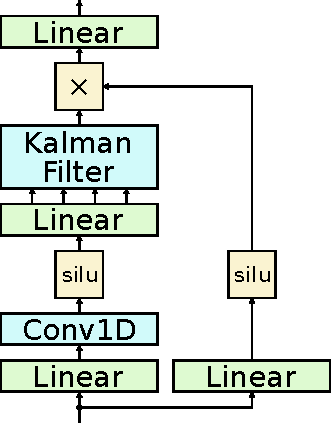
\includegraphics[height=7cm]{Figures/middle_diag.pdf}};

% --- Estimate KF block position within the PDF image ---
% The KF block sits roughly 55-60% up from bottom, on the left portion of the image.
\coordinate (kf-top-left) at ($(img.south west)+(-0.15, 4.95)$);
\coordinate (kf-bot-left) at ($(img.south west)+(-0.15, 3.95)$);

% =============================================
% LEFT SIDE: W matrix (info unroll)
% =============================================
\begin{scope}[shift={($(img.west)+(-10.5, 0.5)$)}, local bounding box=matrixarea]

  % --- Information-unroll matrix W ---
  \node[anchor=north west, font=\small, align=left] (matW) at (0, 2.5) {%
    $\mathbf{W} = \begin{pmatrix}
      k_1 {\color{UncBlue}\Lambda_1^v}
        & 0
        & \cdots
        & 0 \\[4pt]
      {\color{forgetred}f_2}\, k_1 {\color{UncBlue}\Lambda_1^v}
        & k_2 {\color{UncBlue}\Lambda_2^v}
        & \cdots
        & 0 \\[4pt]
      \vdots & \vdots & \ddots & \vdots \\[4pt]
      {\color{forgetred}\textstyle\prod_{s=2}^{T} f_s}\, k_1 {\color{UncBlue}\Lambda_1^v}
        & {\color{forgetred}\textstyle\prod_{s=3}^{T} f_s}\, k_2 {\color{UncBlue}\Lambda_2^v}
        & \cdots
        & k_T {\color{UncBlue}\Lambda_T^v}
    \end{pmatrix}$%
  };

\end{scope}

% =============================================
% BELOW MATRIX: Equations + legend (separate label area)
% =============================================
\begin{scope}[shift={($(matrixarea.south west)+(0, -0.3)$)}, local bounding box=labelarea]

  % --- General element formula ---
  \node[anchor=north west, font=\small, align=left] (geneq) at (0, 0) {%
    $W_{ij} = \begin{cases}
      \displaystyle {\color{forgetred}\prod_{s=j+1}^{i} f_s} \;\cdot\; k_j \,{\color{UncBlue}\Lambda_j^v}
        & \text{if } i \geq j \\[6pt]
      0 & \text{otherwise}
    \end{cases}$%
  };

  % --- M_seq factorization ---
  \node[anchor=north west, font=\small, inner sep=0pt] (mseq) at (0, -1.55) {%
    $\mathbf{M}_{\mathrm{seq}}
      \;=\;
      \mathrm{diag}\!\bigl(
        \mathbf{q} \odot {\color{UncBlue}\boldsymbol{\lambda}^{-1}}
      \bigr)
      \,\mathbf{W}$%
    \qquad\scriptsize\textrm{(output readout \& precision scaling)}%
  };

  % --- Compact vector output equation ---
  \node[anchor=north west, font=\small, inner sep=0pt] (veceq) at (0, -2.15) {%
    $\mathbf{y} \;=\;
      \underbrace{%
        \mathbf{M}_{\mathrm{seq}}\,\mathbf{v}
      }_{\text{\scriptsize attention}}
      +\;
      \underbrace{%
        (\mathbf{q} \odot {\color{UncBlue}\boldsymbol{\lambda}^{-1}})
        \odot \mathbf{b} \odot \boldsymbol{\eta}_0%
      }_{\text{\scriptsize init-state}}$%
  };

  % --- Color legend ---
  \node[anchor=north west, font=\scriptsize, align=left] (legend) at (0, -3.45) {%
    {\color{forgetred}\rule{0.7em}{0.7em}} forget gates $f_s$ \quad
    {\color{UncBlue}\rule{0.7em}{0.7em}} uncertainty $\Lambda^v\!,\;\lambda$ {\small(KLA-only)} \quad
    {\rule{0.7em}{0.7em}} shared with SSM/GLA%
  };

\end{scope}

% =============================================
% CENTER: Expanding cone from KF block to W matrix
% =============================================

% Cone target anchors: top-right and bottom-right of the matrix area only
\coordinate (cone-tr) at (matrixarea.north east);
\coordinate (cone-br) at (matrixarea.south east);

% Fill the cone region
\fill[cyan!4]
    (kf-top-left) -- (cone-tr) -- (cone-br) -- (kf-bot-left) -- cycle;

% Dashed cone lines
\draw[dashed, thick, gray!50] (kf-top-left) -- (cone-tr);
\draw[dashed, thick, gray!50] (kf-bot-left) -- (cone-br);

% "attention view" label along the cone
\node[font=\scriptsize, gray!70, rotate=8]
  at ($(kf-bot-left)!0.45!(cone-tr)+(0, -0.15)$) {\textit{attention view}};

\end{tikzpicture}%
}